\documentclass{standalone}

\usepackage[latin1]{inputenc}
\usepackage{amsmath}
\usepackage{amssymb}
\usepackage{amsthm}

\usepackage{tikz}
\usetikzlibrary{arrows}
\usetikzlibrary{calc}
\usetikzlibrary{snakes}

%% generates a tightly fitting border around the work
%\usepackage[active,tightpage]{preview}
%\PreviewEnvironment{tikzpicture}
%\setlength\PreviewBorder{0.5mm}
%%\renewcommand\PreviewBbAdjust{-\PreviewBorder 1mm -1.15mm -0.85mm}

\usepackage{color}

%\pagestyle{empty}

\begin{document}

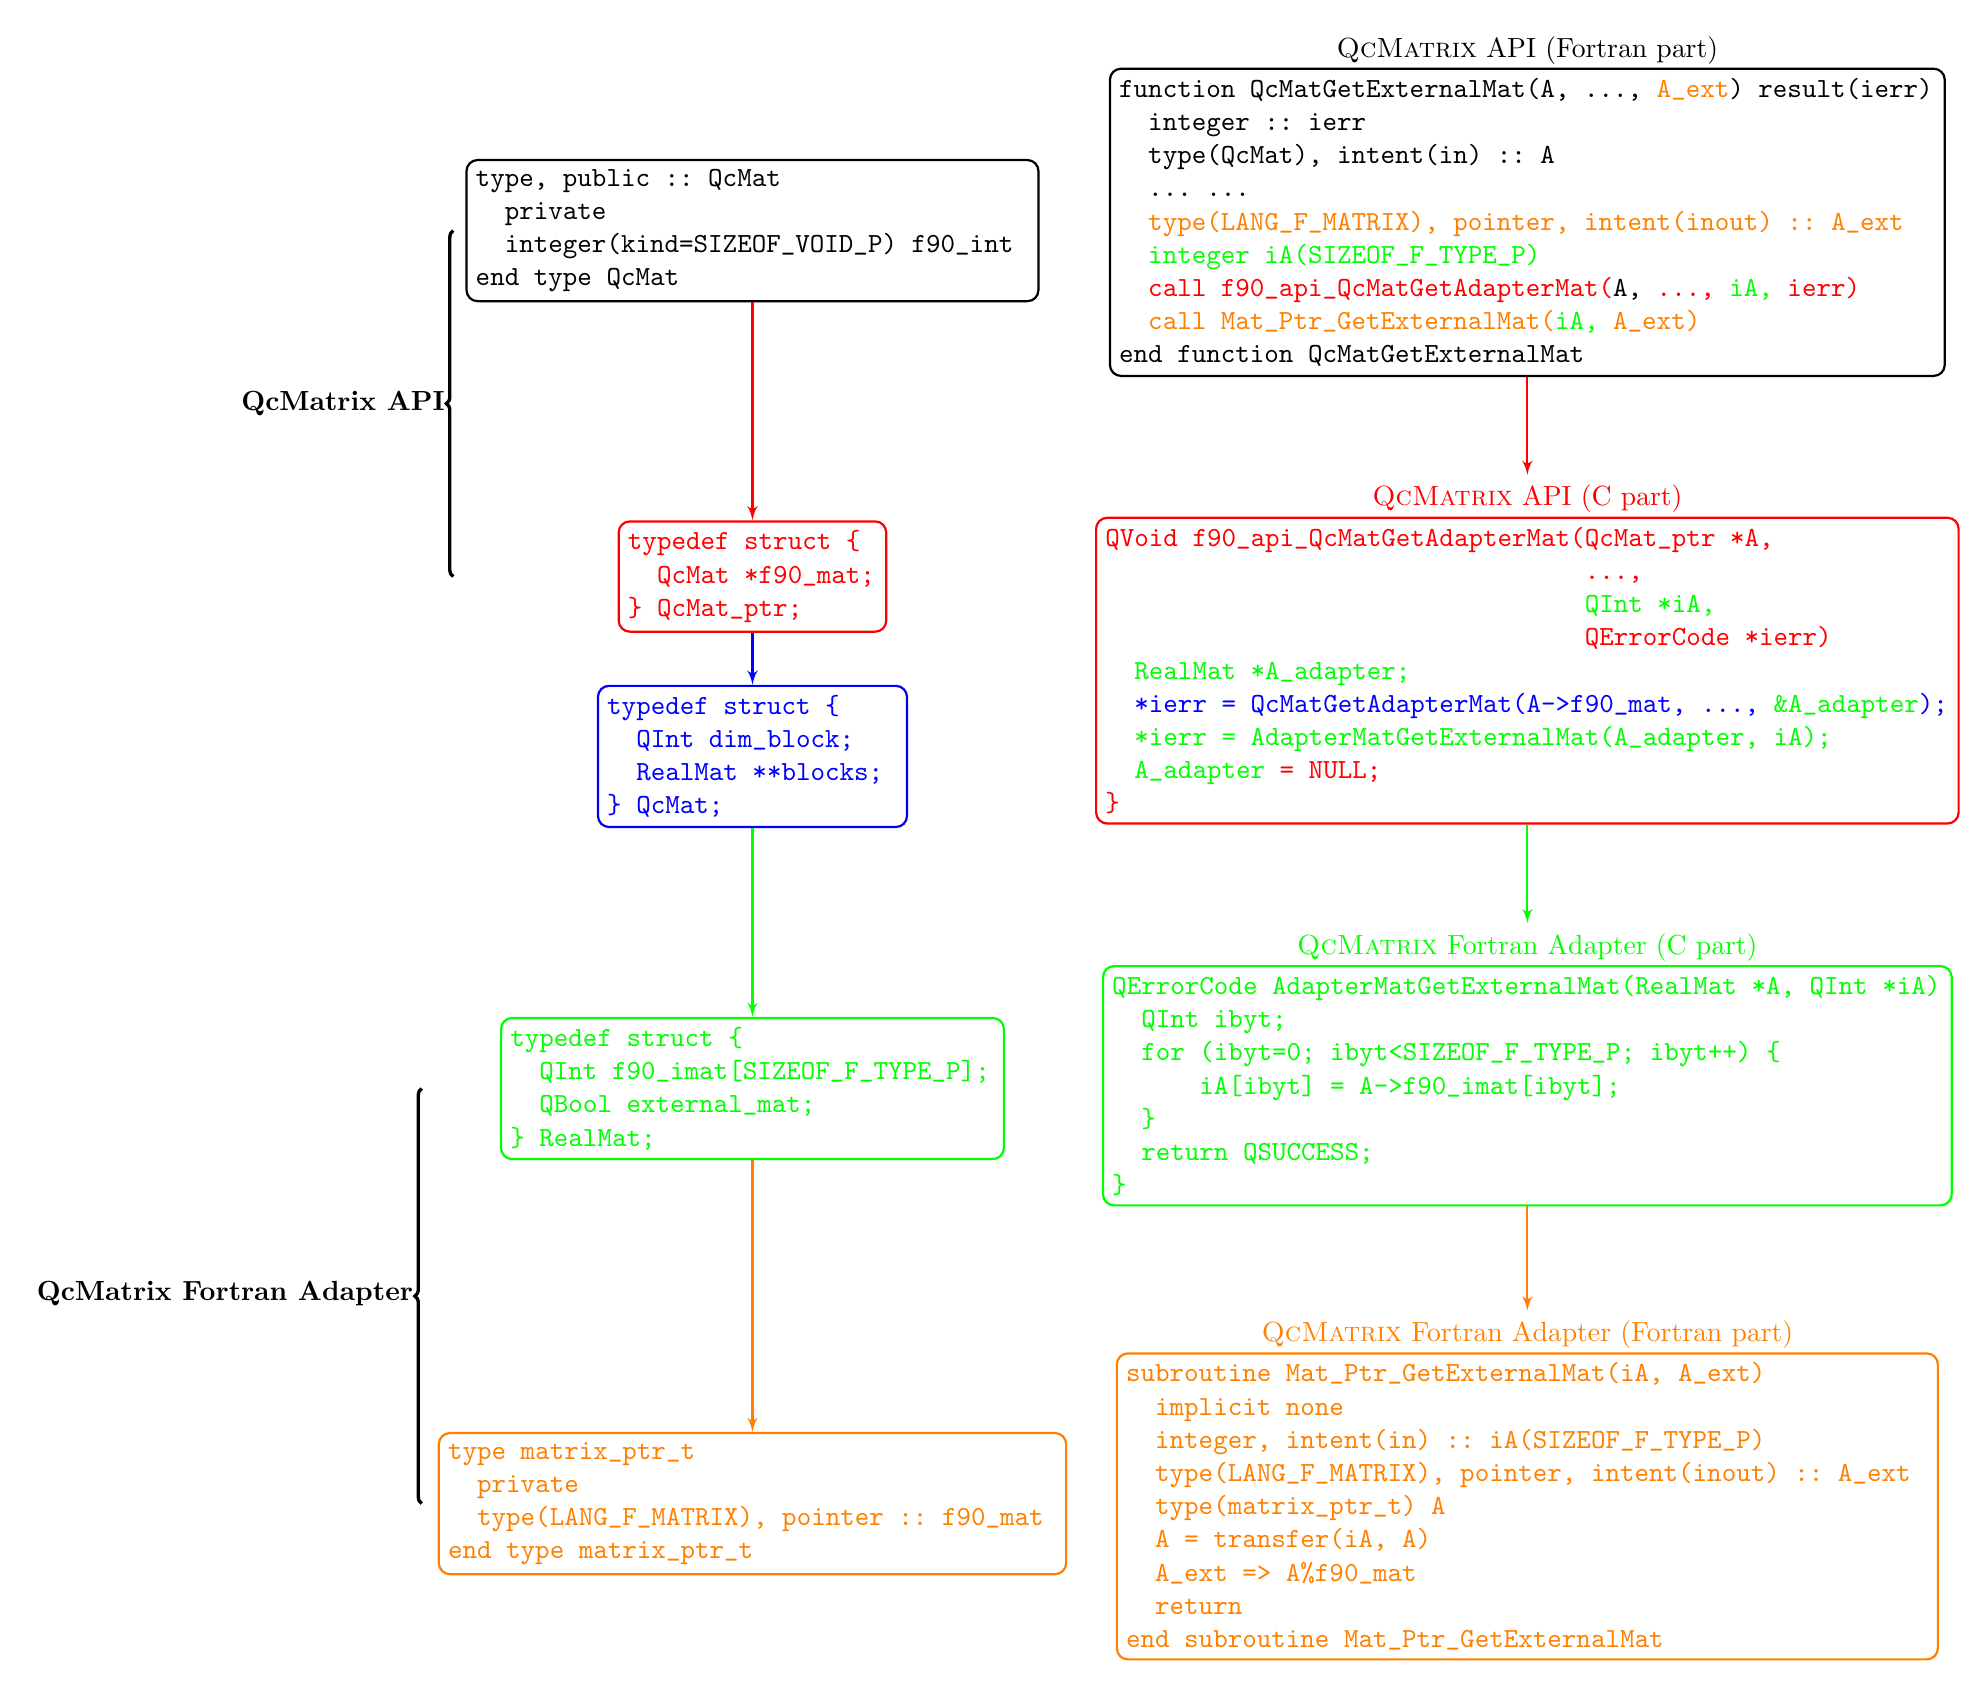
\begin{tikzpicture}[thick]
  % QcMat (Fortran)
  \node[color=black, rectangle, draw, text badly ragged, rounded corners, %
        minimum height=20, text width=200] (QcMatFDef) %
       {\verb|type, public :: QcMat| %
        \linebreak\verb|  private| %
        \linebreak\verb|  integer(kind=SIZEOF_VOID_P) f90_int|
        \linebreak\verb|end type QcMat|};
  % QcMat_ptr
  \node[color=red, rectangle, draw, text badly ragged, rounded corners, minimum height=20,
        text width=90, below of=QcMatFDef, node distance=125] (QcMatPtrDef) %
       {\verb|typedef struct {| %
        \linebreak\verb|  QcMat *f90_mat;| %
        \linebreak\verb|} QcMat_ptr;|};
  \draw [color=red, -latex'] (QcMatFDef)--(QcMatPtrDef);
  \draw [very thick, decoration={brace, mirror}, decorate] ($(QcMatFDef)-(3.8,0)$)--($(QcMatPtrDef)-(3.8,0)$);
  \node at ($(QcMatFDef)-(5.2,2.2)$) {\textbf{\textsc{QcMatrix} API}};
  % QcMat
  \node[color=blue, rectangle, draw, text badly ragged, rounded corners, %
        minimum height=20, text width=105, below of=QcMatPtrDef, node distance=65] (QcMatDef) %
       {\verb|typedef struct {| %
        \linebreak\verb|  QInt dim_block;| %
        \linebreak\verb|  RealMat **blocks;| %
        \linebreak\verb|} QcMat;|};
  \draw [color=blue, -latex'] (QcMatPtrDef)--(QcMatDef);
  % RealMat
  \node[color=green, rectangle, draw, text badly ragged, rounded corners, minimum height=20,
        text width=175, below of=QcMatDef, node distance=120] (RealMatDef) %
       {\verb|typedef struct {| %
        \linebreak\verb|  QInt f90_imat[SIZEOF_F_TYPE_P];| %
        \linebreak\verb|  QBool external_mat;| %
        \linebreak\verb|} RealMat;|};
  \draw [color=green, -latex'] (QcMatDef)--(RealMatDef);
  % matrix_ptr_t
  \node[color=orange, rectangle, draw, text badly ragged, rounded corners, minimum height=20,
        text width=220, below of=RealMatDef, node distance=150] (MatPtrDef) %
       {\verb|type matrix_ptr_t| %
        \linebreak\verb|  private| %
        \linebreak\verb|  type(LANG_F_MATRIX), pointer :: f90_mat| %
        \linebreak\verb|end type matrix_ptr_t|};
  \draw [color=orange, -latex'] (RealMatDef)--(MatPtrDef);
  \draw [very thick, decoration={brace, mirror}, decorate] ($(RealMatDef)-(4.2,0)$)--($(MatPtrDef)-(4.2,0)$);
  \node at ($(RealMatDef)-(6.7,2.6)$) {\textbf{\textsc{QcMatrix} Fortran Adapter}};
  % APIs
  \node[color=black, right of=QcMatFDef, node distance=280, yshift=65] (NoteAPIF) %
       {\textsc{QcMatrix} API (Fortran part)};
  \node[color=black, rectangle, draw, text badly ragged, rounded corners, minimum height=20, % 
        text width=295, below of=NoteAPIF, node distance=62] (APIF) %
       {\verb|function QcMatGetExternalMat(A, ..., |\color{orange}\verb|A_ext|\color{black}\verb|) result(ierr)| %
        \linebreak\verb|  integer :: ierr| %
        \linebreak\verb|  type(QcMat), intent(in) :: A| %
        \linebreak\verb|  ... ...| %
        \linebreak\color{orange}\verb|  type(LANG_F_MATRIX), pointer, intent(inout) :: A_ext| %
        \linebreak\color{green}\verb|  integer iA(SIZEOF_F_TYPE_P)| %
        \linebreak\color{red}\verb|  call f90_api_QcMatGetAdapterMat(|\color{black}\verb|A, |\color{red}\verb|..., |\color{green}\verb|iA, |\color{red}\verb|ierr)| %
        \linebreak\color{orange}\verb|  call Mat_Ptr_GetExternalMat(|\color{green}\verb|iA, |\color{orange}\verb|A_ext)| %
        \linebreak\color{black}\verb|end function QcMatGetExternalMat|};
  \node[color=red, below of=APIF, node distance=100] (NoteAPIC) {\textsc{QcMatrix} API (C part)};
  \node[color=red, rectangle, draw, text badly ragged, rounded corners, minimum height=20, % 
        text width=305, below of=NoteAPIC, node distance=62] (APIC) %
       {\verb|QVoid f90_api_QcMatGetAdapterMat(QcMat_ptr *A,| %
        \linebreak\verb|                                 ...,| %
        \linebreak\color{green}\verb|                                 QInt *iA,| %
        \linebreak\color{red}\verb|                                 QErrorCode *ierr)| %
        \linebreak\color{green}\verb|  RealMat *A_adapter;| %
        \linebreak\color{blue}\verb|  *ierr = QcMatGetAdapterMat(A->f90_mat, ..., |\color{green}\verb|&A_adapter|\color{blue}\verb|);| %
        \linebreak\color{green}\verb|  *ierr = AdapterMatGetExternalMat(A_adapter, iA);| %
        \linebreak\verb|  A_adapter|\color{red}\verb| = NULL;| %
        \linebreak\verb|}|};
  \draw [color=red, -latex'] (APIF)--(NoteAPIC);
  % adapater
  \node[color=green, below of=APIC, node distance=100] (NoteAdapterC) %
       {\textsc{QcMatrix} Fortran Adapter (C part)};
  \node[color=green, rectangle, draw, text badly ragged, rounded corners, minimum height=20, % 
        text width=300, below of=NoteAdapterC, node distance=50] (AdapterC) %
       {\verb|QErrorCode AdapterMatGetExternalMat(RealMat *A, QInt *iA)| %
        \linebreak\verb|  QInt ibyt;| %
        \linebreak\verb|  for (ibyt=0; ibyt<SIZEOF_F_TYPE_P; ibyt++) {| %
        \linebreak\verb|      iA[ibyt] = A->f90_imat[ibyt];| %
        \linebreak\verb|  }| %
        \linebreak\verb|  return QSUCCESS;| %
        \linebreak\verb|}|};
  \draw [color=green, -latex'] (APIC)--(NoteAdapterC);
  \node[color=orange, below of=AdapterC, node distance=90] (NoteAdapterF) %
       {\textsc{QcMatrix} Fortran Adapter (Fortran part)};
  \node[color=orange, rectangle, draw, text badly ragged, rounded corners, minimum height=20, % 
        text width=290, below of=NoteAdapterF, node distance=62] (AdapterF) %
       {\verb|subroutine Mat_Ptr_GetExternalMat(iA, A_ext)| %
        \linebreak\verb|  implicit none| %
        \linebreak\verb|  integer, intent(in) :: iA(SIZEOF_F_TYPE_P)| %
        \linebreak\verb|  type(LANG_F_MATRIX), pointer, intent(inout) :: A_ext| %
        \linebreak\verb|  type(matrix_ptr_t) A| %
        \linebreak\verb|  A = transfer(iA, A)| %
        \linebreak\verb|  A_ext => A%f90_mat| %
        \linebreak\verb|  return| %
        \linebreak\verb|end subroutine Mat_Ptr_GetExternalMat|};
  \draw [color=orange, -latex'] (AdapterC)--(NoteAdapterF);
\end{tikzpicture}

\end{document}
